\documentclass{report}
\usepackage{color}
\usepackage{times}
\usepackage{natbib}
\usepackage{float}

\usepackage{Sweave}
\begin{document}
\title{Stroke Documentation using \LaTeX{} }
\author{Pouria Mojabi, \texttt{mojabi@genophen.com}}
\date{\today}
\maketitle


\section{Introduction}
This Documentation is intended for Strok Disease. all the risk factors that are associated with Stroke are identified and assesed. 
From genitics to your daily routines. Calculations are primarily based on two sources. CDC(NHANES) dataset and scientific papers. 
Some risk factors are extracted from CDC and some are extracted from the papers. Below you will find details about each risk factor. 
risk Factors from NHANES dataset can all be found under CDC section.
references can be found at the end of the document

\newpage
\section{\color{blue} Diabetes}
Diabetes is a categorical variable with binary state. Either yes or no wheter you have it or not \newline
\begin{tabular}{ | l | c || r |}
\hline
Diabetes & OR & CI\\ \hline
No & 1 & ref \\ \hline
Yes & 2.78 & 2.13-3.61\\ \hline
\end{tabular}
\newline \newline
Values of this table are from \citet{shahar2003} paper.

\newpage
\section{\color{blue}Blood Pressure}
After consulting with Dr.Malek we decide to implement 
\citet{Kim2005}. {\bf \color{red} Note that population is Asian only}. on the website we should present this with a disclaimer.
\newline \newline
\begin{tabular}{|l|l|l|l|l|l|l|}
\hline
Category & Optimal & Normal & HighNormal & HypertensionI & HypertensionII & HypertensionIII \\ \hline
SBP & <120 & 120-129 & 130-139 & 140-159 & 160-179 & >180 \\ \hline
OR & 1 & 1.43 & 1.81 & 2.82 & 3.91 & 6.58\\ \hline
CI & 1.16-1.76 & 1.47-2.23 & 2.31-3.41 & 3.09-4.95 & 4.96-8.73\\ \hline
\end{tabular}
\newline \newline \newline \newline
\begin{tabular}{|l|l|l|l|l|l|l|}
\hline
Category & Optimal & Normal & HighNormal & HypertensionI & HypertensionII & HypertensionIII \\ \hline
DBP & <80 & 80-84 & 85-89 & 90-99 & 100-109 & >110 \\ \hline
OR & 1 & 1.43 & 1.81 & 2.82 & 3.91 & 6.58\\ \hline
CI & 1.16-1.76 & 1.47-2.23 & 2.31-3.41 & 3.09-4.95 & 4.96-8.73\\ \hline
\end{tabular}
\newline 
{\bf *Normal range is considered baseline and optimal range gives a protective effect*}
Les see some graphs!
\begin{figure}[b!]
\centering
\includegraphics{EPFL-BP}
\caption{OR vs BP}
\end{figure}


\newpage
\section{\color{blue}SleepCondition}
Not getting proper sleep can increase the probability of getting a Stroke. Odds ratios are taken from \cite{Dyken2009}
\newline \newline
\begin{tabular}{|l|l|l|}
\hline
SleepCondition & OR & CI\\ \hline
Sleep Apnea & 2.89 & 1.3-6.09\\ \hline
Sleep Disorder & 2.89 & 1.37-6.09\\ \hline
\end{tabular}


\newpage
\section{\color{blue}Past CVD Condition}
This considered your family history. ORs are extracted from \cite{Pullicino2009} and Shoshana Reshef (couldn't find this, check with sadaf)
\newline \newline
\begin{tabular}{|l|l|l|}
\hline
PastCVD & OR & CI\\ \hline
Atrail Fibrilation & 2.86 & 1.25-6.58\\ \hline
Myocardial Infaction & 2.09 & 1.23-3.55\\ \hline
HeartFailure and Stroke & 2.2 & 1.5-3.4\\ \hline
\end{tabular}


\newpage
\section{\color{blue}CDC}
Some risk factors are calculated using NHANES dataset. Logistic regression is performed and odds ratios are calculated. 
we will briefly mention the model below.
{\color{red} Y-axis of all the Plots is log scale(log of odds ratio)}
\begin{Schunk}
\begin{Soutput}
Call:
glm(formula = CVD ~ BMIC2 + Age + Gender + WaistAdBMI2 + Race, 
    family = binomial, data = Data1)

Deviance Residuals: 
    Min       1Q   Median       3Q      Max  
-0.7320  -0.2955  -0.1613  -0.0837   3.8650  

Coefficients:
              Estimate Std. Error z value Pr(>|z|)    
(Intercept)  -9.252646   0.777788 -11.896  < 2e-16 ***
BMIC2         0.064821   0.011524   5.625 1.85e-08 ***
Age3          1.883263   0.759363   2.480  0.01314 *  
Age4          2.720815   0.726350   3.746  0.00018 ***
Age5          3.495981   0.719462   4.859 1.18e-06 ***
Age6          4.099682   0.713808   5.743 9.28e-09 ***
Age7          4.473912   0.713955   6.266 3.70e-10 ***
Age8          5.147710   0.712539   7.224 5.03e-13 ***
GenderM      -0.075031   0.103354  -0.726  0.46786    
WaistAdBMI2   0.019773   0.007346   2.692  0.00711 ** 
Race2Hisp     0.010918   0.118142   0.092  0.92637    
Race3NHBlack  0.441559   0.112831   3.913 9.10e-05 ***
Race4Other    0.330240   0.252858   1.306  0.19154    
---
Signif. codes:  0 ‘***’ 0.001 ‘**’ 0.01 ‘*’ 0.05 ‘.’ 0.1 ‘ ’ 1 

(Dispersion parameter for binomial family taken to be 1)

    Null deviance: 5077.3  on 18866  degrees of freedom
Residual deviance: 4381.9  on 18854  degrees of freedom
AIC: 4407.9

Number of Fisher Scoring iterations: 9
\end{Soutput}
\end{Schunk}
\newpage
Lets take a look at our Base Model 
\begin{Schunk}
\begin{Sinput}
> layout(matrix(c(1, 2, 3, 4), 2, 2))
> plot(Mbase)
\end{Sinput}
\end{Schunk}
\begin{figure}[H]
\centering
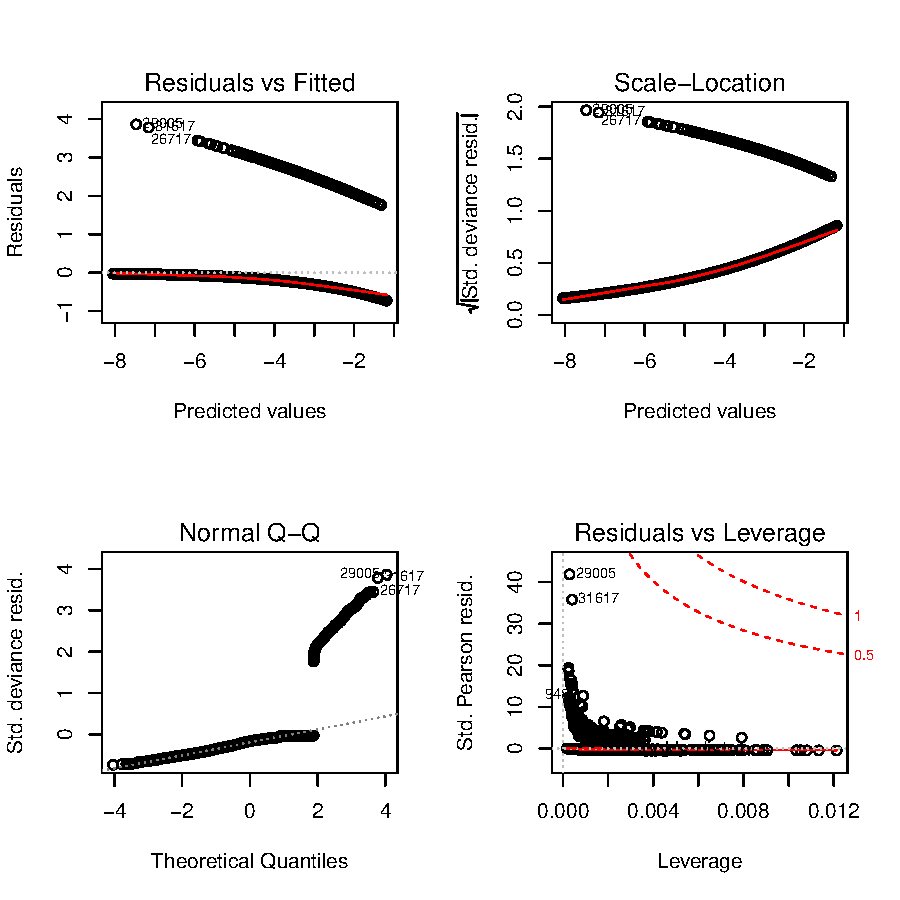
\includegraphics{EPFL-Mbase}
\caption{Logistic Regression}
\end{figure}

\newpage
\subsection{\color{green}BMI}
BMI is calculated directly from CDC dataset;
\begin{center}
\begin{figure}[H]
\includegraphics{EPFL-BMI}
\caption{OR ratio vs BMI}
\end{figure}
\end{center}

\newpage
\subsection{\color{green}Age}
Age (a categorical variable in this case) can directly get caluclated from the base model
\begin{center}
\begin{figure}[H]
\includegraphics{EPFL-Age}
\caption{OR vs Age}
\end{figure}
\end{center}

\newpage
\subsection{\color{green}Gender}
Gender is also a categorical variable. either Male or Female can't be both!
\begin{center}
\begin{figure}[H]
\includegraphics{EPFL-Gender}
\caption{OR ratio vs Gender}
\end{figure}
\end{center}

\newpage
\subsection{\color{green}AdjustedWaist}
Since BMI and Waist are highly correlated, together they can't contribute to the prediction. Infact Waist can be predicted by BMI,
linear regression results in : 
Waist = 2.74 * BMI - 16.9
AdjustedWaist is the difference between an actual Waist and the predicted waist from BMI (basically the error)
so, we have:
WaistAdjustedBMI = waist - 2.74 * BMI + 16.9
\begin{center}
\begin{figure}[H]
\includegraphics{EPFL-adwaist}
\caption{OR vs AdjustedWaist}
\end{figure}
\end{center}

\newpage
\subsection{\color{green}Trig}
Without further do we present the plot here that shows the Odds ratio with differen Trig values
\begin{figure}[H]
\includegraphics{EPFL-trig}
\caption{OR vs Trig}
\end{figure}


\newpage
\subsection{\color{green}Smoking}
Well, obviously smoking is bad for you! this should depict how bad it could be
\begin{figure}[H]
\includegraphics{EPFL-smk}
\caption{OR vs Smoking}
\end{figure}





\bibliographystyle{plain}
\bibliography{papers}
\end{document}
